\documentclass[WHATMANUAL.tex]{subfiles}

\begin{document}

\section{What is WHAT}

WHAT (Well Hydrograph Analysis Toolbox) is a free, open source, and cross-platform interactive computer program whose main focus is the interpretation of observation well hydrographs. It is written in the Python 2.7 programming language and is currently maintained and developed by Jean-Sébastien Gosselin at INRS-ETE (\url{www.ete.inrs.ca}). The source code and a stand-alone executable for Windows~7 are available free of charge for download on GitHub (\url{www.github.com/jnsebgosselin/WHAT}).

If you encounter any problems or errors during program execution, have any questions, or have suggestions on how to improve WHAT, please contact Jean-Sébastien Gosselin at this email address: \href{mailto:jnsebgosselin@gmail.com}{jnsebgosselin@gmail.com}.

\section{Features}

Below are listed the features that are available in the current version of WHAT, as well as the ones that are going to be incorporated in future versions of the software.

\paragraph*{Features available in current version of WHAT :}

\begin{itemize}

\item Gapless Daily Weather Time Series Preparation :
   
    \begin{itemize}    
        \item Graphical interface to the online Canadian Daily Climate Database (CDCD) to search for weather station by location coordinate.
        \item Automatic downloading and formatting of available data from the CDCD.
        \item Estimation of missing data and automatic gapfilling of the datasets.
    \end{itemize}
 
\item Data Visualization:

    \begin{itemize}
        \item Data exploration in a user-friendly and dynamic graphical environment.
        \item Production of publication-quality graphs in vectorial formats (pdf or svg).
    \end{itemize}

\item Weather Data Analysis :

    \begin{itemize}
        \item Estimation of yearly and monthly normals.
        \item Estimation of the daily potential evapotranspiration.
    \end{itemize}

\item Water Level Analysis :

    \begin{itemize}
        \item Calculation of the master recession curve (MRC).
        \item Estimation of groundwater recharge from the MRC using a continuous water-table fluctuation (WTF) method.
    \end{itemize}

\end{itemize}

\paragraph*{Features planned for future versions of WHAT :}

\begin{itemize}

\item Synthetic hydrograph production for the estimation of groundwater recharge and prediction of water levels.

\item Assessment of the level of confinement of the aquifer at the well location based on an analysis of the barometric response function of the water level record.

\end{itemize}

\section{Installation}\label{sec:intallation}

WHAT can run on Windows, Linux, or OS~X computer operating systems. However, a stand-alone executable of the program is currently released and tested only for the Windows~7 platform. This executable should also be compatible with Windows~XP. For the Linux and OS~X platforms, the software can be run directly from the source code, provided that Python~2.7 and all the required third party packages are installed on the computer (PySide, NumPy, matplotlib, xlrd, xlwt).

The stand-alone executable for Windows~7 is distributed in a Zip archive that can be downloaded freely on GitHub (\url{https://github.com/jnsebgosselin/WHAT/releases}). This archive contains:

\begin{itemize}

\item the GNU General Public License;

\item a folder named ``WHAT'' that contains all the necessary system files for the program to run, including the file ``WHAT.exe'' from which the software can be started;

\item a folder named ``Projects'' where all input and output files used or created by WHAT are stored by default. This folder includes samples of input and output files that provide a quick and convenient way to test and learn the various features of the program.

\end{itemize}

Once the content of the Zip archive has been extracted, the program can be started directly from the ``WHAT.exe'' executable file that is contained within the folder named ``WHAT''. The software can conveniently run from any location on the computer or from any storage device without the need to install the program beforehand.

\section{Overview of the Graphical User Interface}
\label{sec:GUI_overview}

%There is no traditional menus in WHAT and everything is instead displayed within a menu bar that is located at the top of the interface.

The Graphical User Interface (GUI) of WHAT mainly consists of a menu bar, a console area, and a central view panel (\cref{fig:WHAT_GUI}). The \emph{menu bar} is located in the top right corner of the GUI. This is where the name of the current project is displayed and where it is possible to open an existing project or create a new one. The \emph{console} is located at the bottom of the GUI and is used to report technical information about the various tasks accomplished by the program as well as warning and error messages. The console can be collapsed vertically to save space, or can be extended to the entire window area. The \emph{central view panel} is the main component of the GUI. It is where the various features of the software are displayed. The content of this panel is divided into four tabs: \emph{Download Data}, \emph{Fill Data}, \emph{Hydrograph}, and \emph{About}. These tabs are described in more details below and are shown in \cref{fig:WHAT_GUI_ScnShot}.

\begin{figure}[!hb]
    \setlength{\fboxsep}{0pt}
    \ffigbox[\FBwidth]
    {
     \caption{Screenshot of WHAT v4.1.7-beta in Ubuntu-Linux 15.04 showing the \emph{About} tab.}
     \label{fig:WHAT_GUI}
    }
    {
     \fbox{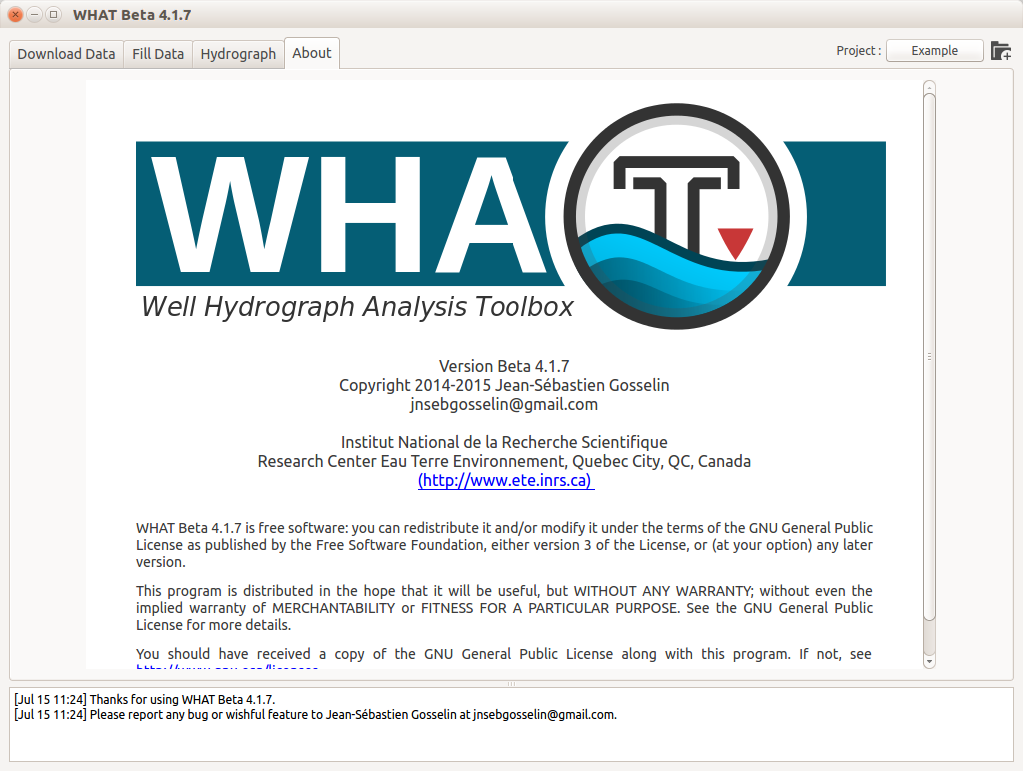
\includegraphics[width=0.75\textwidth]{img/WHAT_GUI}}
    }
\end{figure}

\newpage

\paragraph{Download Data :} This tab (\cref{subfig:ScnShot_000}) provides a graphical interface to the online Canadian Daily Climate Database (CDCD), owned and operated by Environment Canada, from which it is possible to interactively search for stations by location coordinates, download the available data, and automatically organize the data in a format compatible with WHAT.

\begin{figure}[!ht]
    \centering
    \begin{subfigure}[t]{0.45\textwidth}
        \setlength{\fboxsep}{0pt}
        \fbox{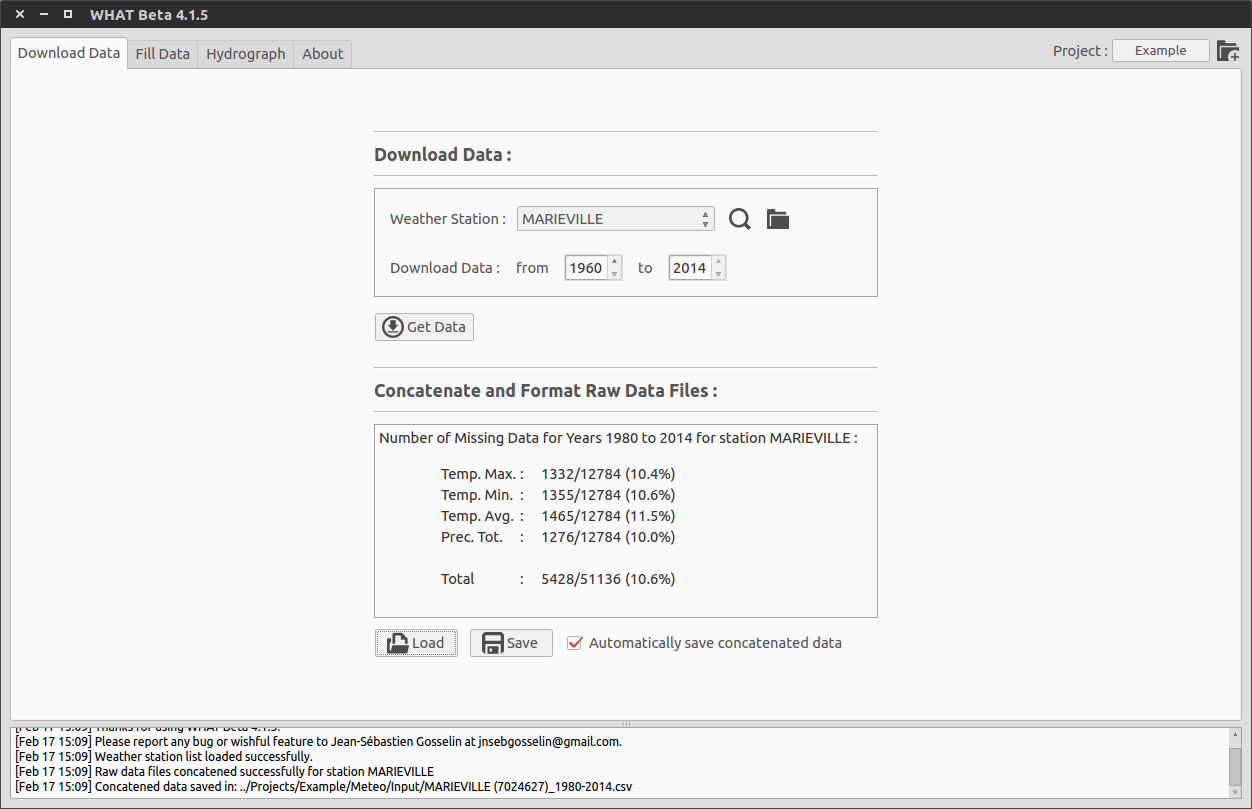
\includegraphics[width=\textwidth]{img/WHAT_Screenshot000}}
        \caption{\emph{Download Data} tab.}
        \label{subfig:ScnShot_000}                
    \end{subfigure}%
    \hspace{0.5cm}
    \begin{subfigure}[t]{0.45\textwidth}
        \setlength{\fboxsep}{0pt}
        \fbox{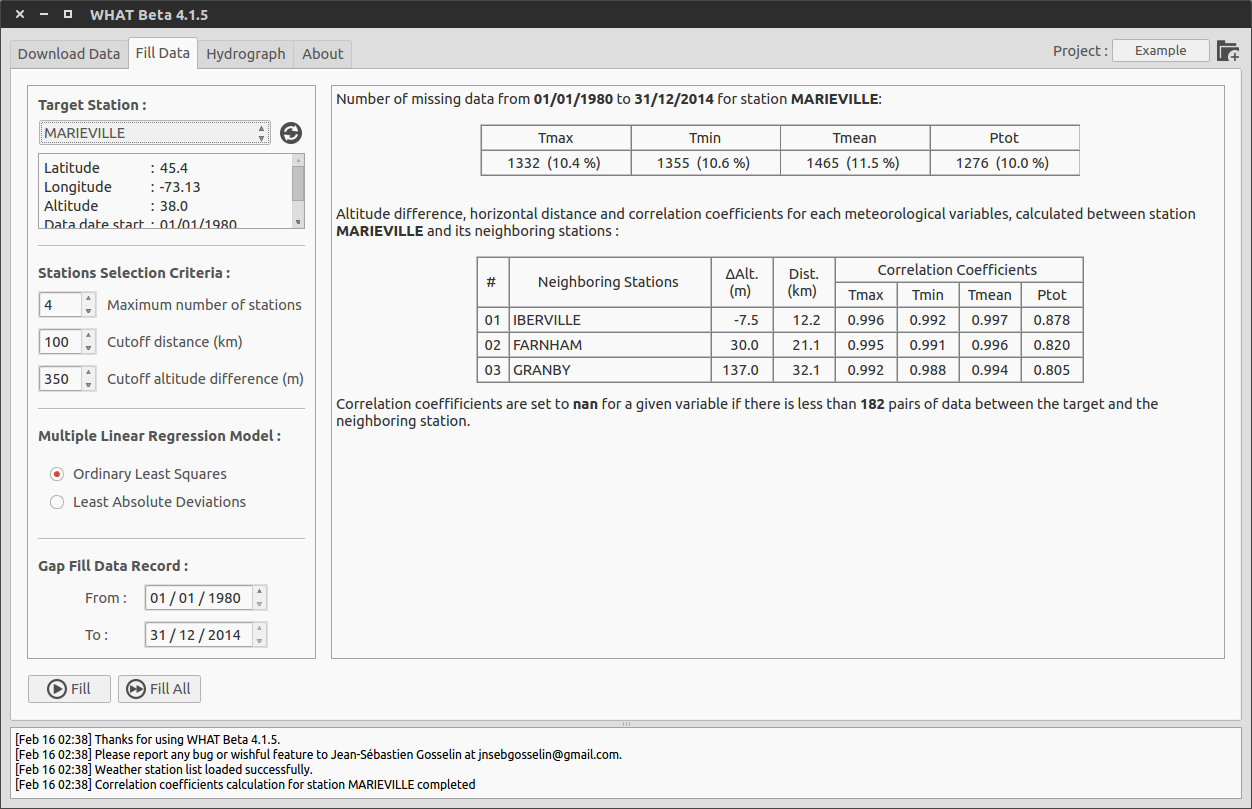
\includegraphics[width=\textwidth]{img/WHAT_Screenshot001}}
        \caption{\emph{Fill Data} tab.}
        \label{subfig:ScnShot_001}
    \end{subfigure}
    \\[0.5cm]
    \begin{subfigure}[t]{0.45\textwidth}
        \setlength{\fboxsep}{0pt}
        \fbox{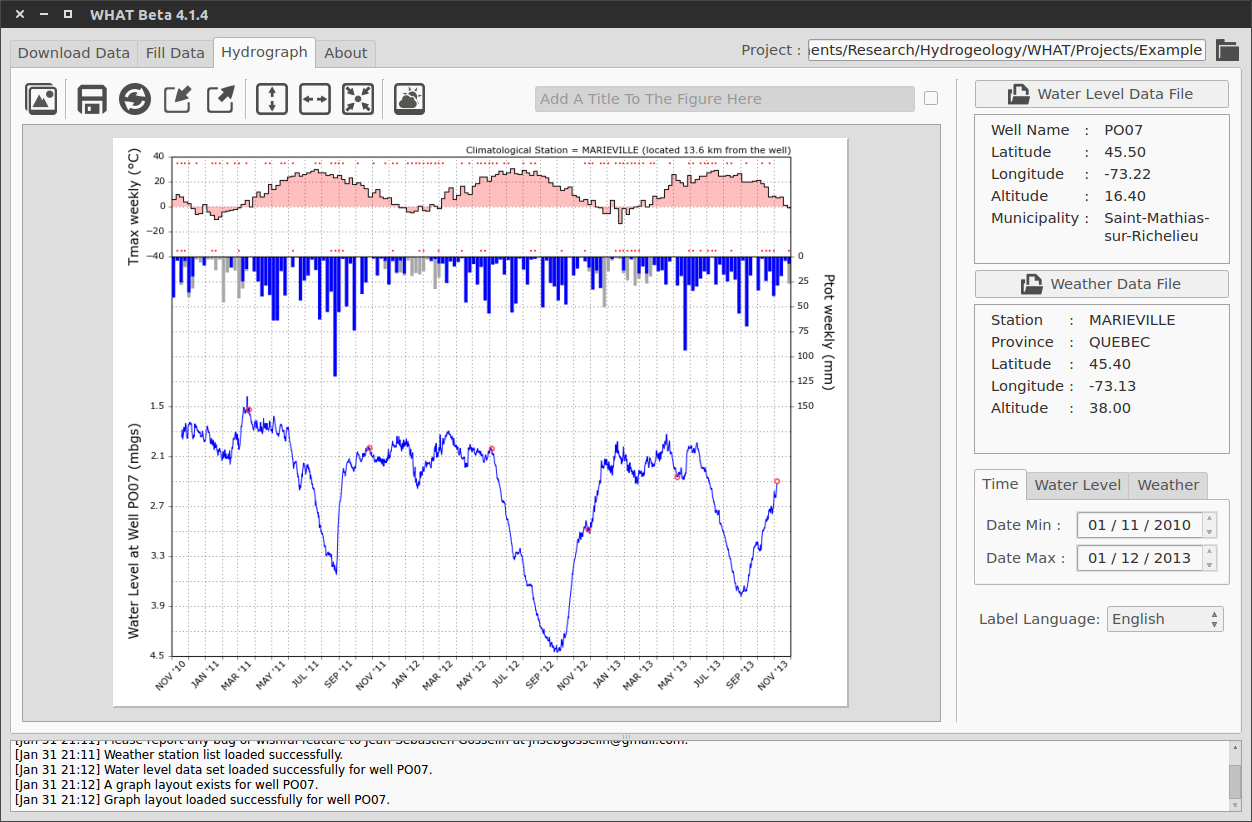
\includegraphics[width=\textwidth]{img/WHAT_Screenshot002}}
        \caption{\emph{Hydrograph} tab in \emph{Layout} mode.}
        \label{subfig:ScnShot_002}
    \end{subfigure}
    \hspace{0.5cm}
    \begin{subfigure}[t]{0.45\textwidth}
        \setlength{\fboxsep}{0pt}
        \fbox{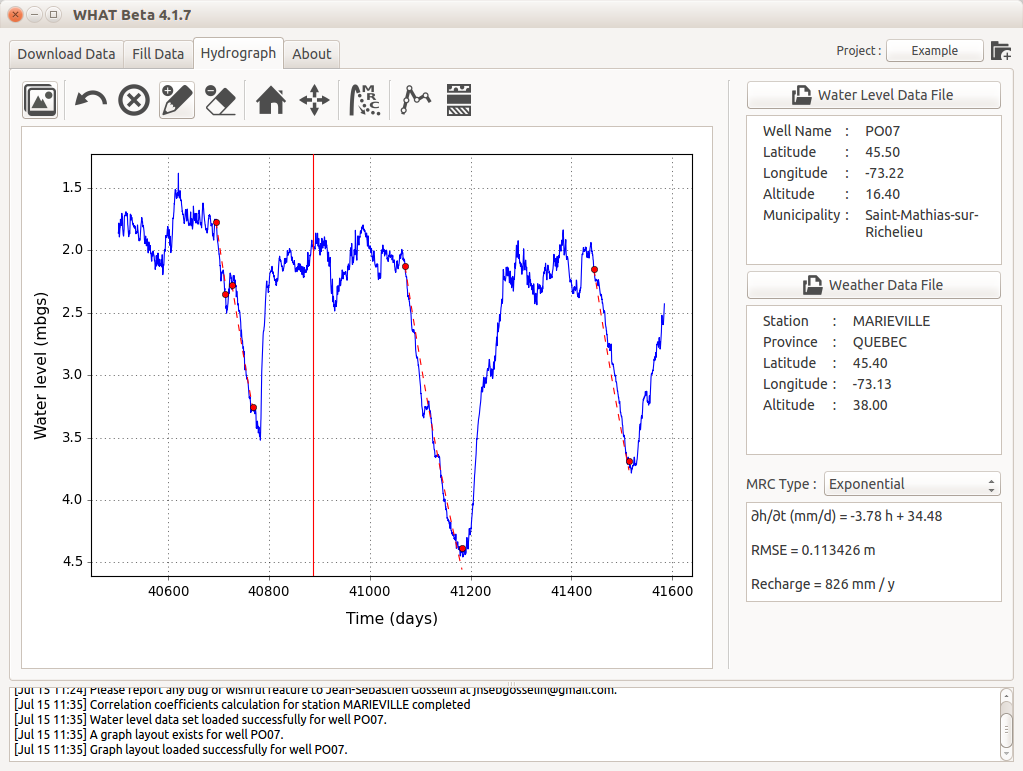
\includegraphics[width=\textwidth]{img/WHAT_Screenshot003}}
        \caption{\emph{Hydrograph} tab in \emph{Computation} mode.}
        \label{subfig:ScnShot_003}
    \end{subfigure}
    \caption[Screenshots of WHAT v4.1.7-beta captured in Ubuntu Linux 15.04.]{Screenshots of WHAT v4.1.7-beta captured in Ubuntu Linux 15.04. showing : (a) the \emph{Download Data} tab, (b) the \emph{Fill Data} tab (c) the \emph{Hydrograph} tab in \emph{Layout} mode, and (d) the \emph{Hydrograph} tab in \emph{Computation} mode.}\label{fig:WHAT_GUI_ScnShot}
\end{figure}

\paragraph{Fill Data :} This tab (\cref{subfig:ScnShot_001}) provides an automated procedure to estimate and fill the missing values in the daily weather datasets. Missing data in a dataset from a given station are estimated with data from selected neighboring weather stations using a multiple linear regression model.

\paragraph{Hydrograph :} This tab is used for viewing and plotting both groundwater level and weather time series. For this purpose, two modes are available: the \emph{layout} and the \emph{computation} mode. Both modes share the same weather and water level datasets and it is possible to switch from one mode to the other at anytime. The \textbf{layout} mode (\cref{subfig:ScnShot_002}) provides a graphical interface to interactively produce publication-quality graphs. The \textbf{computation} mode (\cref{subfig:ScnShot_003}) consists in a dynamic graphical environment where data can be visualized, manipulated and analyzed. Various computational tools are available in this mode, including the estimation of the Master Recession Curve (MRC) and the estimation of groundwater recharge.

\paragraph{About :} This tab (\cref{fig:WHAT_GUI}) displays copyright, licensing and general information about WHAT.

%\section{Workflow for Interpreting Water-level Time-series}\label{sec:workflow}
%
%WHAT is a computer software that brings together a set of tools to assist the interpretation of water level time series, from the processing of raw data to the assessment of groundwater recharge. Some are well known and documented techniques such as the estimation of missing daily weather values with the use of a multiple regression model. Others are genuine improvements of not well known or used method, such as the estimation of groundwater recharge using an approach based on the fitting of a synthetic hydrograph to real groundwater level measurements. Furthermore, WHAT has been design from the start to be modular, meaning that it will be very easy to add more tools in the future to expand the possibilities of this software.
%
%The strength of WHAT lies not only in its various tools, but in the integration of these into a complete functional workflow for the interpretation of water level time series. This workflow is presented in Figure~\ref{fig:WHAT_workflow}. By providing a unique centralized environment where data can be processed, explored and analyzed, a lot of data manipulation and time can be saved. Moreover, the interpretation of the data is facilitated greatly, thanks to the dynamical graphical environment that is provided within the software. This is a significant improvement over the use of fragmented tools and methods, some of which are often no more than a generic spreadsheet that are not well suited for the dynamical exploration of time series.
%
%\begin{figure}
%\centering
%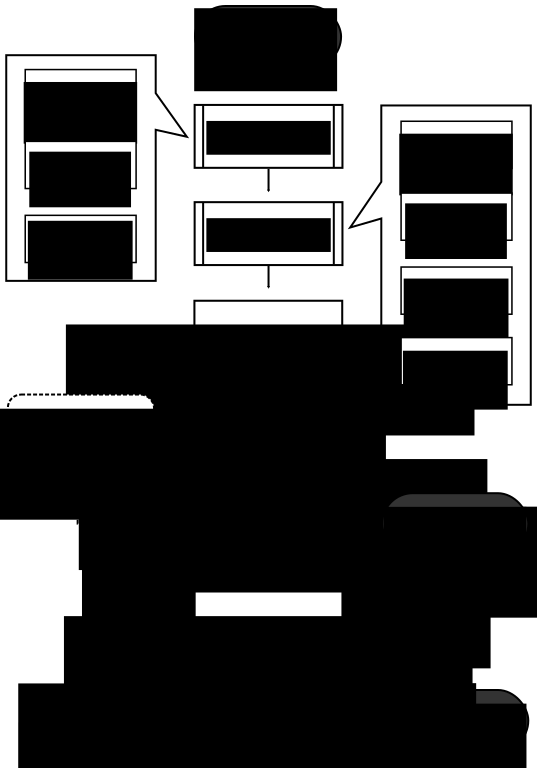
\includegraphics[height=0.95\textheight]{img/WHAT_Workflow}
%\caption[WHAT workflow.]{WHAT workflow for the interpretation of groundwater-level time-series measured in an observation well or a piezometer.}
%\label{fig:WHAT_workflow}
%\end{figure}
%
%The workflow shown in Figure~\ref{fig:WHAT_workflow} represents the interpretation of the data for only one well at one particular location. But, WHAT is also well suited for regional characterization projects that requires the management of data from multiple locations within a large study area. More specifically, the software allows to navigate easily through the different water level and weather datasets related to a given study area and makes the comparison of the data and the mass production of graphs and analyses efficient and easy. This can represent a substantial gain in time and data manipulation when the number of well for a given study area is important and when there is a need to update the data multiple times over the course of the project. Details about the management of projects in WHAT is presented in Section~\ref{WHAT_projects}.
%
%The first step in the proposed workflow of Figure~\ref{fig:WHAT_workflow} for the interpretation of water level time series is the preparation of gapless weather datasets. This include downloading and formatting weather data from the CDCD database and estimating the missing daily values within each record by using data from selected neighboring stations. This step is covered in details in Section~\ref{chap:gapfilling}. The second step is the processing of the water level time series, including the validation and correction of the data. This is covered in details in Section~\ref{chap:wlvl_formatting}.
%
%Once the weather and water level time series have been prepared, the next step consists in the production of the well hydrographs. This step is covered in details in Section~\ref{chap:plotting_data}. The plotting of the water level and weather data time-series is an important step in the interpretation process that should not be looked down since it can provide meaningful insights about the confinement conditions of the aquifer at the local and regional scale. For example, Appendix~\ref{app:confinement_cond_in_MontEst} presents an application where well hydrographs produced with an early version of WHAT were used to qualitatively deduced the confinement conditions of the regional bedrock aquifer in Monteregie Est($\sim$9000~km\textsuperscript{2}) located in southern Quebec, Canada \citep{carrier_portrait_2013}. The results from this qualitative analysis showed good agreement with the map of confinement conditions of the regional bedrock aquifer which was based on the sequence and thickness of the surficial deposits. 
%
%Following the production of the well hydrographs, if the water level and barometric measurements were acquired at a sufficient sampling rate, it is then possible to calculate the barometric response function of the well \citep{butler_jr._new_2011,rasmussen_identifying_1997,spane_considering_2002}. This tool is very useful to characterized the confinement conditions of the aquifer around the well and also gives meaningful insights about the transmissivity of the well. This approach is discussed in Section~\ref{chap:BRF} and an example of an application to the Monteregie Est area is presented in Appendix~C base on a poster presentation by Gosselin et al.
%
%Using the drill log of the well, the hydrograph, and the barometric response function, it should be possible to determine with a good degree of confidence if the well is in confined or unconfined conditions. For the latter case, the water level and weather data time series can be used jointly to asses the groundwater recharge of the aquifer. The first step of this task consists in the estimation of the Master Recession Curve (MRC) of the hydrograph. In the second step, groundwater recharge is estimated as the residual of a daily soil moisture balance (DSMB) model and the resulting fluxes are substituted into a mathematical model of the aquifer groundwater balance to produce a synthetic well hydrograph. The third and final step of the method consists in the calibration of the DSMB model parameters, based on the comparison of synthetic and observed well hydrographs. An example of groundwater recharge estimation is provided in Appendix~D for a well located at Rougemont in Monteregie Est, Quebec, Canada.

\end{document}


%\begin{itemize}
%
%\item The preparation of gapless daily weather time-series (total precipitation and air temperature), including:
%    
%    \begin{itemize}
%        \item A graphical interface to query the online Canadian Daily Climate Database (CDCD) for weather stations by location coordinates, download the available data for the selected stations, and automatically organize the data in a format compatible with WHAT.
%                
%        \item An automated, robust, and efficient algorithm to quickly and easily fill the gaps in the dataset from a given station by using data from selected neighboring stations.
%    \end{itemize}
%
%\item Various tools to generate publication-quality graphs from the weather and water level datasets.
%
%\item A user-friendly and dynamic graphical environment to visualization the data.
%
%\item The calculation of the master recession curve (MRC) of the well hydrograph and the estimation of groundwater recharge using a continuous water-table fluctuation approach.
%
%\end{itemize}
%
%\paragraph*{Features planned for future versions of WHAT:}
%
%\begin{itemize}
%
%\item The estimation of groundwater recharge with a method consisting in the optimization of a daily water surface budget to the water level time series measured in the Well. The sdaily water surface budget uses as input the gapless daily weather datasets that can be generated directly with WHAT.
%
%\item The assessment of the level of confinement of the aquifer at the well location based on the barometric response function of the well \citep{butler_jr._new_2011,bohling_kansas_2011}.
%
%\end{itemize}